\section{Problem (7)}
	A $2.5 \ kg$ block moves in a straight line on a horizontal frictionless surface under the influence of a force that varies with position as shown the figure. How much work is done by the force as the block moves from the origin to $x = 8.0 \ m$?

	\begin{figure}[H]
		\begin{center}
			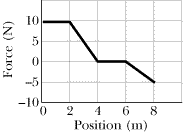
\includegraphics[scale=1]{hw7_problem7}
			\caption{Illustration of Problem 7}
			\label{fig:hw7_problem7}
		\end{center}
	\end{figure}

	\textbf{R:}

	\begin{align}
		W_{(0 \ m \ \to \ 2 \ m)} = \ &(10 \ N)(2 \ m) = 20 \ J& \notag \\
		W_{(2 \ m \ \to \ 4 \ m)} = \ &\frac{1}{2}(10 \ N)(2 \ m) = 10 \ J& \notag \\
		W_{(4 \ m \ \to \ 6 \ m)} = \ &0& \notag \\
		W_{(6 \ m \ \to \ 8 \ m)} = \ &\frac{1}{2}(-5 \ N)(2 \ m) = -5 \ J& \notag \\
		W_{net} = \ &\sum W = 20 \ J + 10 \ J - 5 \ J& \notag \\
		= \ &25 \ J&
	\end{align}
